\documentclass{beamer}
\usepackage{graphicx}
\usepackage{hyperref}

\usetheme[subsectionpage=progressbar]{metropolis}

\title{On Being a Research Computer Scientist}
\subtitle{or what it's like to be a lifelong learner}
\date{November 15\textsuperscript{th}, 2018}
\author{Anthony J. Christe}
\institute{University of Hawaii at Manoa \\ Slippery Rock University of Pennsylvania}

\begin{document}
\maketitle

\section{Introduction}
\begin{frame}{What People Think I Do}
\begin{figure}
	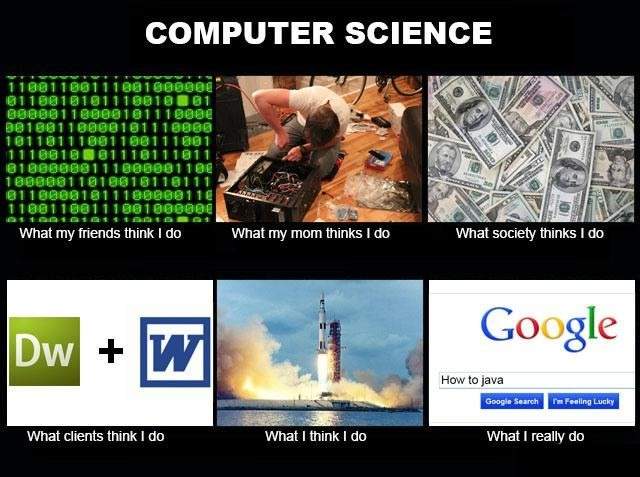
\includegraphics[width=\linewidth]{img/whatido.jpg}
\end{figure}
\end{frame}

\begin{frame}{What I actually do}
\begin{itemize}
	\item Working to obtain PhD in Computer Science
	\begin{itemize}
		\item With an emphasis on Big Data
		\item Distributed sensor networks
		\item Distributed computing
	\end{itemize}
	\item Research Assistant for Infrasound Laboratory
	\begin{itemize}
		\item Design and develop systems for capture, analysis, and reporting of infrasonic signals of interest
	\end{itemize}
\end{itemize}
\end{frame}

\section{How I Got Here}
\begin{frame}{Summary of My Life Until Now}
\begin{itemize}
	\item Graduated High School
	\begin{itemize}
		\item Somerset, PA 2007
	\end{itemize}
	\item B.S. in Computer Science (w/ minor in Theatre)
	\begin{itemize}
		\item Slippery Rock University of PA, 2011
	\end{itemize}
	\item M.S. in Computer Science
	\begin{itemize}
		\item University of Hawaii at Manoa, 2015
	\end{itemize}
	\item Ph.D. in Computer Science
	\begin{itemize}
		\item University of Hawaii at Manoa, Present
	\end{itemize}
\end{itemize}
\end{frame}

\subsection{High School}
\begin{frame}{High School}
\begin{itemize}
	\item No Formal Education in Computer Science
	\item Some self taught Python
	\item Web technologies for cool AIM profiles
	\item Band Geek
	\item Theater Geek
\end{itemize}
\end{frame}

\subsection{Undergraduate Education}
\begin{frame}{Slippery Rock University of Pennsylvania}
	\begin{columns}
		\begin{column}{.34\textwidth}
			\begin{itemize}
				\item Small class sizes
				\item \emph{Close} to home
				\item Ski slope
				\item State school
			\end{itemize}
		\end{column}
		\begin{column}{.66\textwidth}
			\begin{figure}
				
\includegraphics[width=\linewidth]{img/sru.jpg}
			\end{figure}
		\end{column}
	\end{columns}
\end{frame}

\begin{frame}{Slippery Rock University of Pennsylvania}
\begin{figure}
	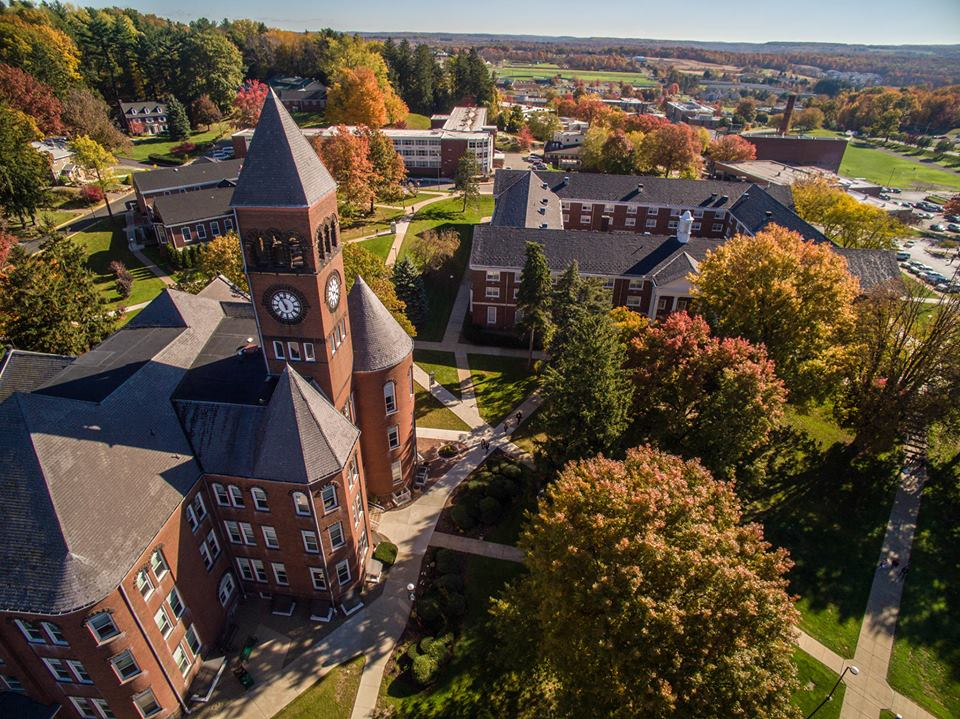
\includegraphics[width=\linewidth]{img/sru2.jpg}
\end{figure}
\end{frame}

\begin{frame}{Slippery Rock University of Pennsylvania}
\begin{figure}
	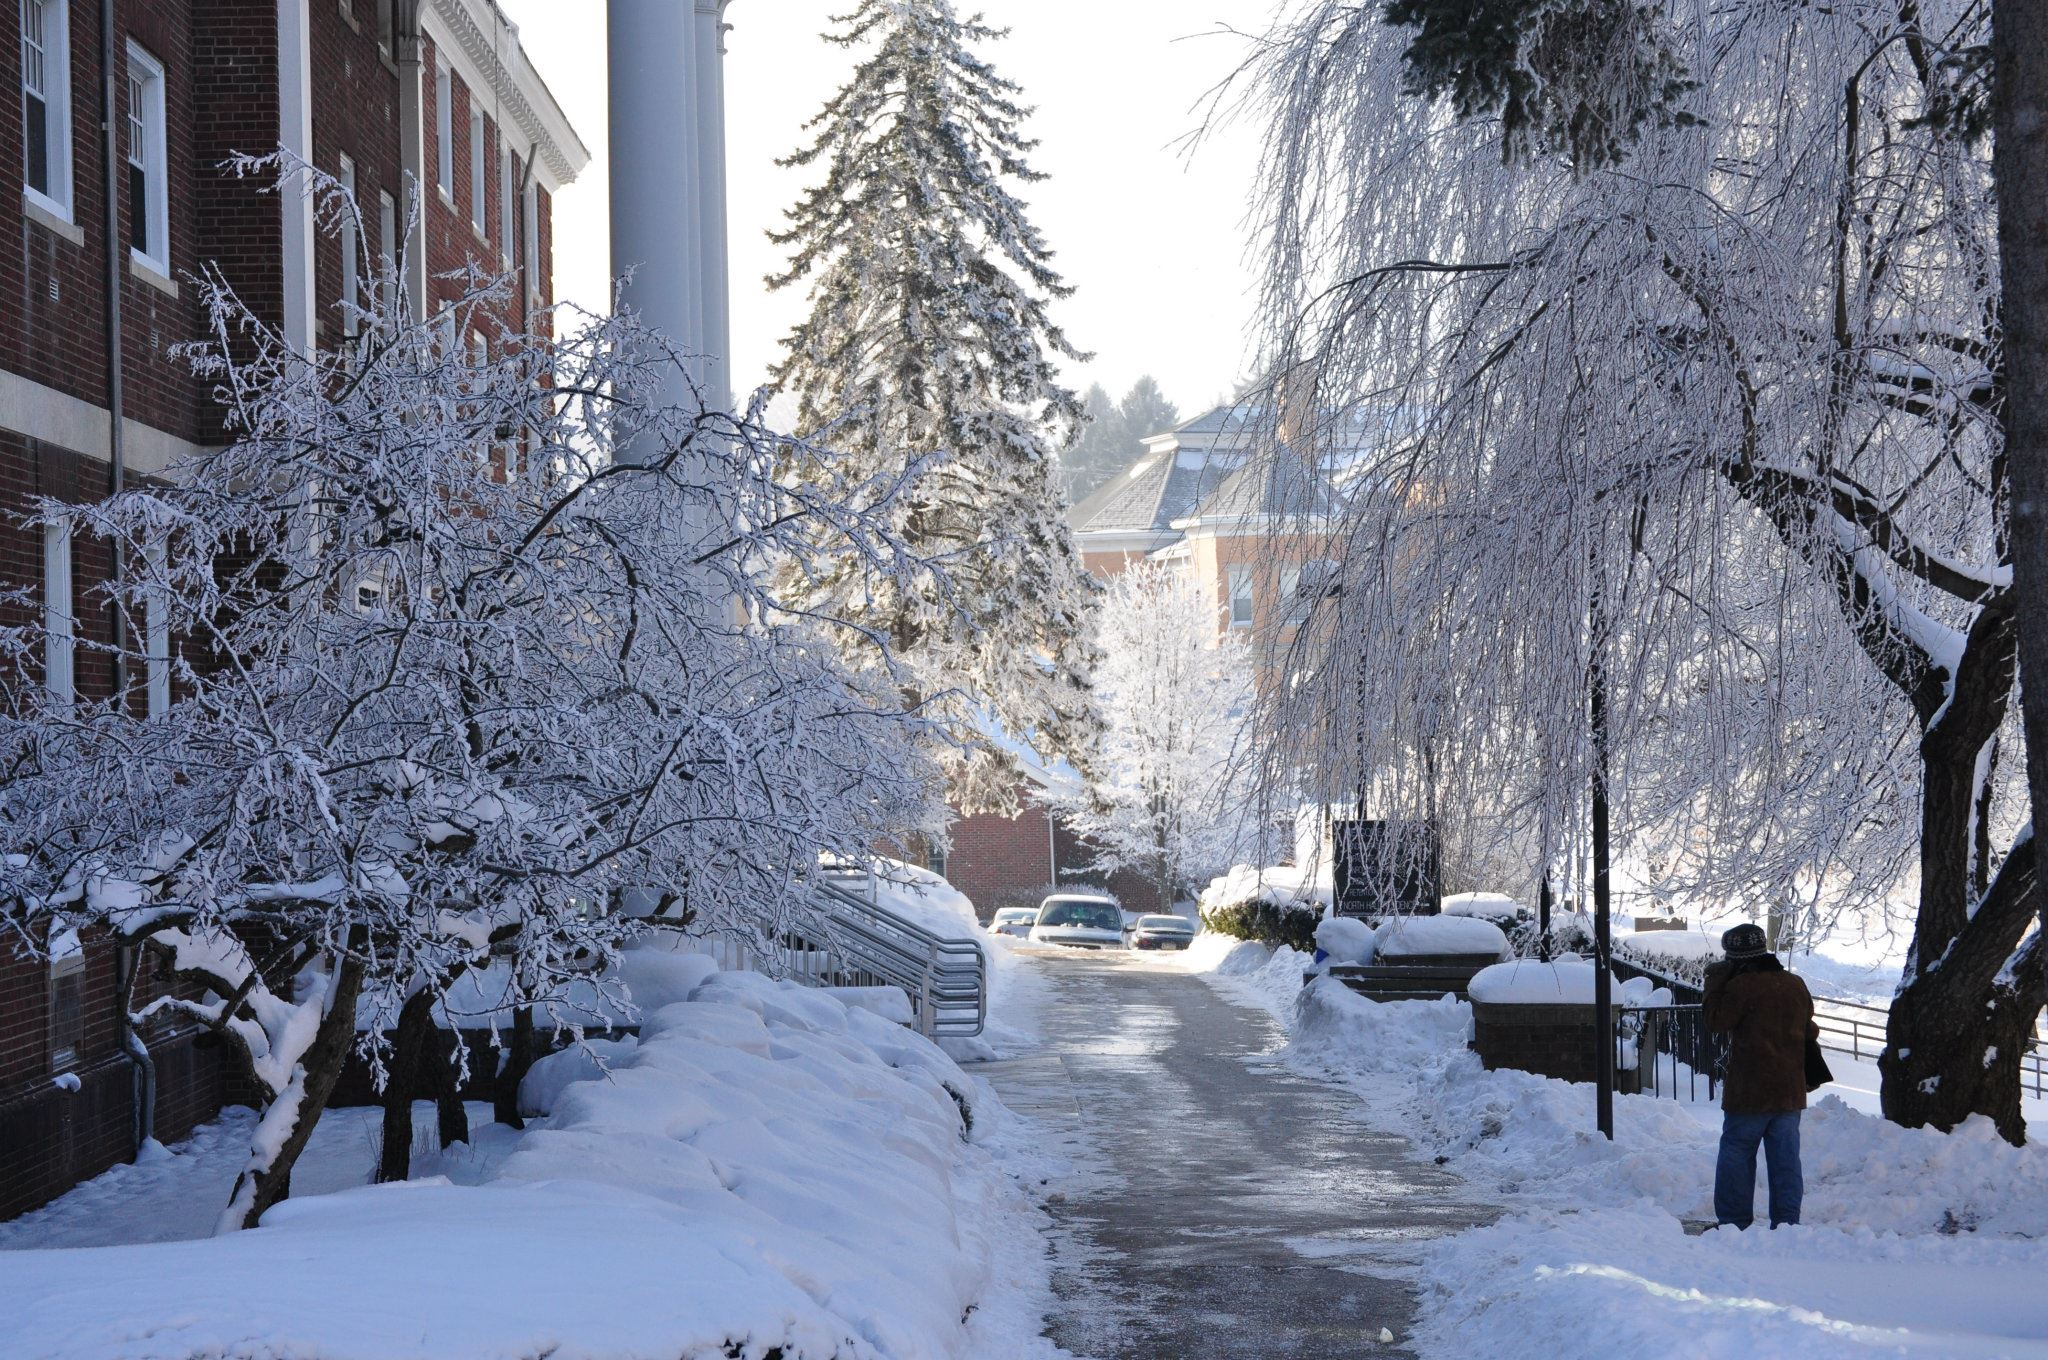
\includegraphics[width=\linewidth]{img/sru4.jpg}
\end{figure}
\end{frame}

\begin{frame}{Artificial Intelligence Robot}
\begin{itemize}
	\item Used genetic algorithms to \emph{teach} a robot to pick up a ball
	\item Machine vision/image processing utilized to find the ball
	\item Wrote a script interpreter
	\begin{itemize}
		\item Programming language for the robot
		\item Could perform movements in parallel
	\end{itemize}
	\item \url{https://www.youtube.com/watch?v=xoBVfaHHHcI}
\end{itemize}
\begin{figure}
	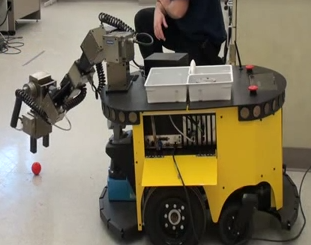
\includegraphics[width=.45\linewidth]{img/robot.png}
\end{figure}
\end{frame}

\begin{frame}{Boulders Computer Cluster}
\begin{itemize}
	\item Used 8 recycled Intel blade servers to build a computer cluster
	\item A single master server managed all slave nodes
	\item Operating system loaded on each slave via PXE
	\item HPC via message passing interface (MPI)
	\begin{itemize}
		\item MapReduce
		\item Apache Spark
		\item \emph{...and many more...}
	\end{itemize}
\end{itemize}
\end{frame}

\begin{frame}{Other Undergrad Activities}
\begin{columns}
	\begin{column}{.50\textwidth}
		\begin{itemize}
			\item Vice-president of $\Upsilon\Pi$E
			\item President of Computer Technology Club
			\item Student Advisor to the Dean
			\item Minor in Theatre
		\end{itemize}
	\end{column}
	\begin{column}{.50\textwidth}
		\begin{figure}
			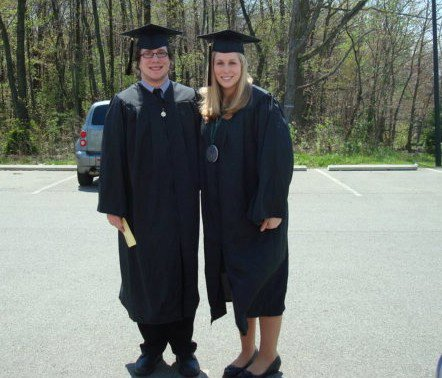
\includegraphics[width=\linewidth]{img/chrissie.jpg}
		\end{figure}
	\end{column}
\end{columns}
\end{frame}

\begin{frame}{After Graduation}
\begin{figure}
	
\includegraphics[width=\linewidth]{img/uh.png}
\end{figure}
\end{frame}

\subsection{Graduate School}

\begin{frame}{What is Graduate School?}
\begin{itemize}
	\item Education beyond your bachelor's degree
	\begin{itemize}
		\item Masters, Ph.D, M.D., Ed.D., \emph{etc}
	\end{itemize}
	\item Generally funded through teaching/research assistantship
	\item Specialization of your field
	\item Research focused
	\item Expects publishing and attending conferences
	\item Novel contribution to the field (Ph.D.)
\end{itemize}
\end{frame}

\begin{frame}{Master's Degree}
	\begin{itemize}
		\item Specialization in your field
		\item Comprehensive project \emph{or}
		\item Master's thesis
		\item Graduate classes
	\end{itemize}
\end{frame}

\begin{frame}{Teaching Assistantship (TA)}
\begin{itemize}
	\item ICS 211 - Intro. to Programming II
	\begin{itemize}
		\item 5 Semesters
		\item Run programming lab
		\item Design homework assignments (sometimes)
		\item Grade homework assignments
		\item Run lecture (when needed)
	\end{itemize}
\end{itemize}
\end{frame}

\begin{frame}{Research Assistantship (RA)}
\begin{itemize}
	\item Paid to perform research 
	\begin{itemize}
		\item Income \textasciitilde\$25,000/yr
		\item Tuition waver \textasciitilde\$22,000/yr
	\end{itemize}
	\item Many more opportunities than a TA
	\item OpenPowerQuality - 1 Semester
	\item Infrasound Laboratory - Current
\end{itemize}
\end{frame}

\begin{frame}{OpenPowerQuality (OPQ)}
	\begin{columns}
		\begin{column}{.50\textwidth}
			\begin{itemize}
				\item Open source distributed sensors and framework
				\begin{itemize}
					\item Detects PQ problems
					\item Stores raw data in cloud
					\item Performs analytics
					\item Reports PQ info to users
				\end{itemize}
			\end{itemize}
		\end{column}
		\begin{column}{.50\textwidth}
			\begin{figure}
				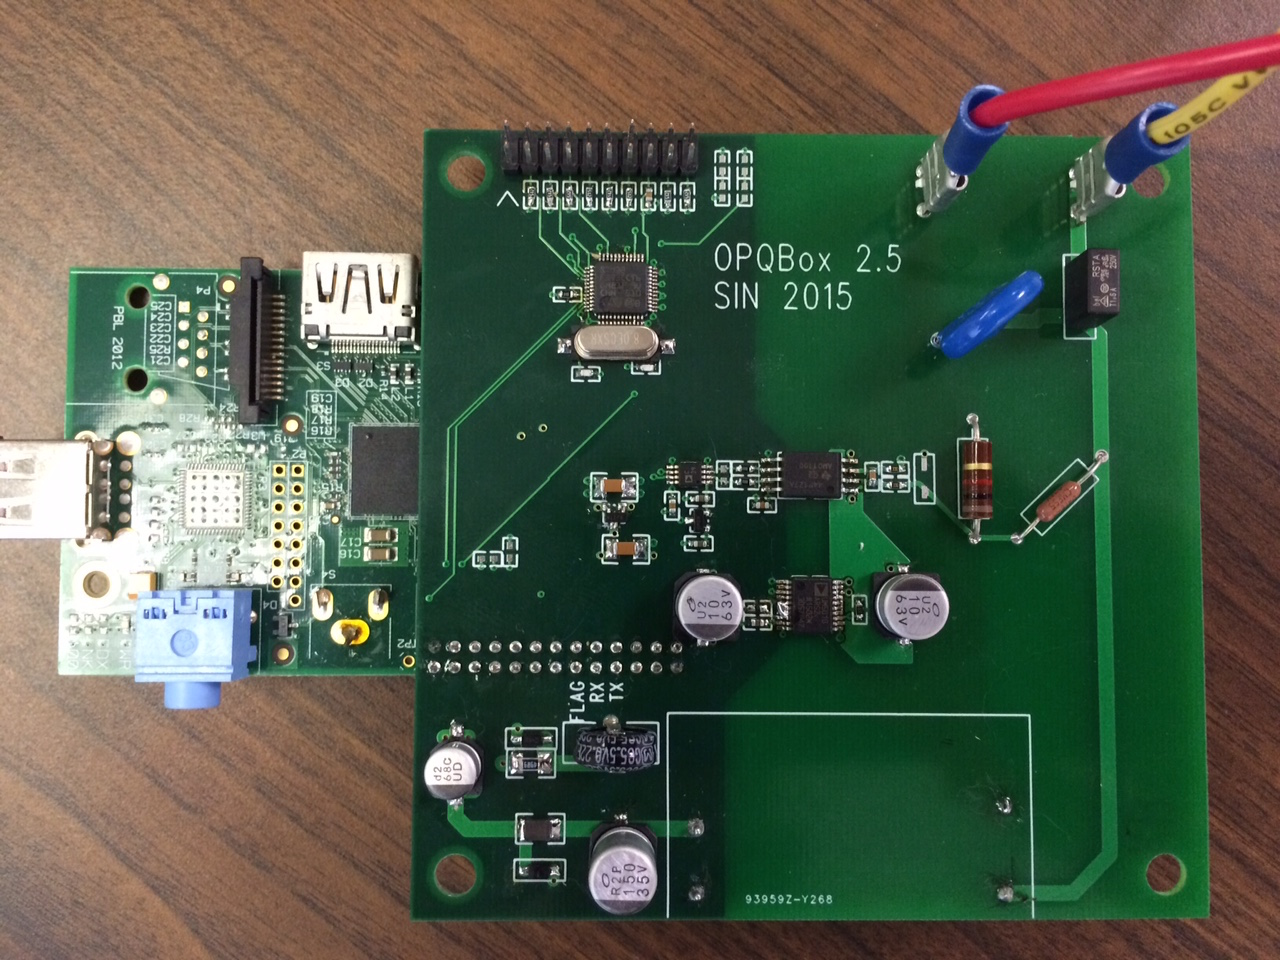
\includegraphics[width=\linewidth]{img/box.JPG}
			\end{figure}
		\end{column}
	\end{columns}
\end{frame}

\begin{frame}{Infrasound Laboratory}
\begin{columns}
	\begin{column}{.60\textwidth}
		\begin{itemize}
			\item Sound $<$20 Hz
			\item Generated by large movements of air
			\begin{itemize}
				\item Volcanoes
				\item Explosions
				\item Storms
				\item Aircraft
				\item Rockets
			\end{itemize}
		\end{itemize}
	\end{column}
	\begin{column}{.40\textwidth}
		\begin{figure}
			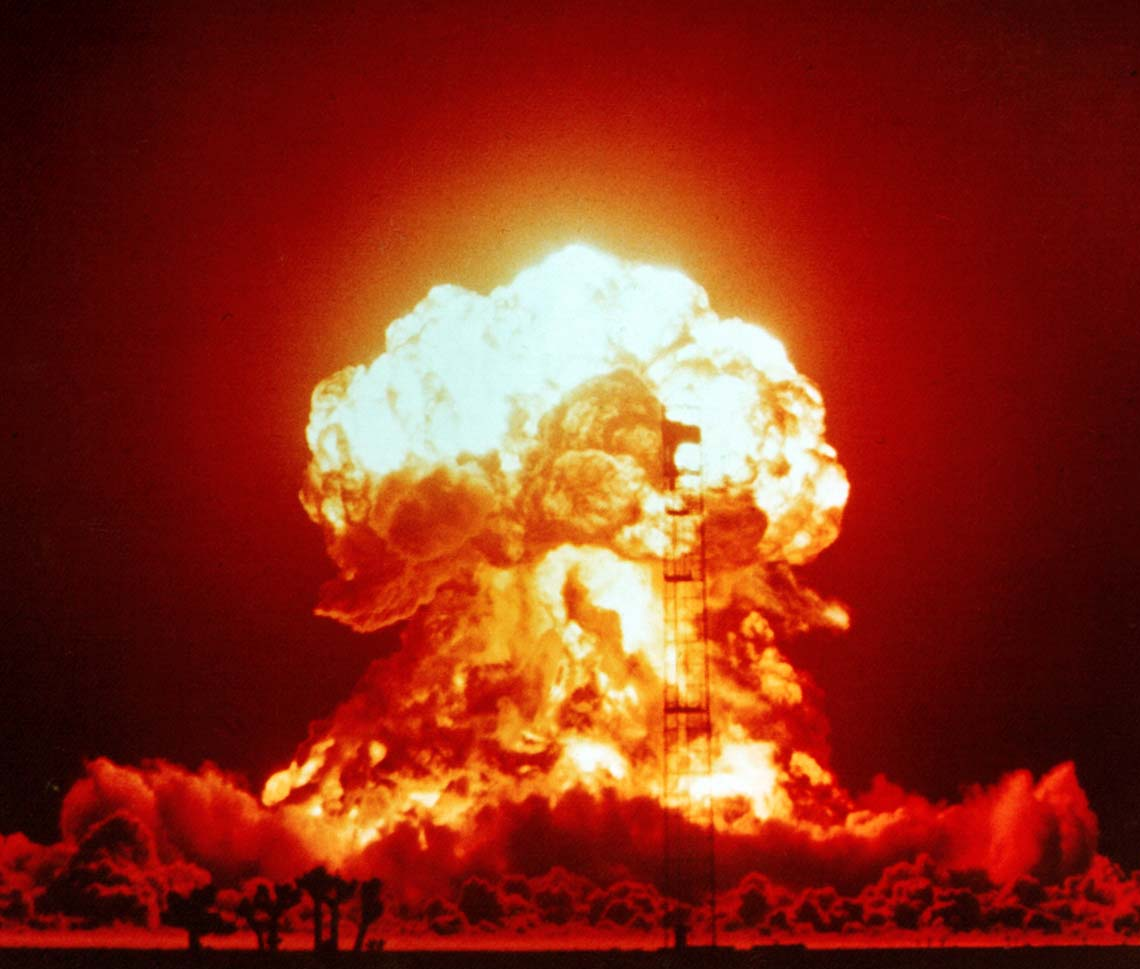
\includegraphics[width=\linewidth]{img/nuke.jpg}
		\end{figure}
	\end{column}
\end{columns}
\end{frame}

\begin{frame}{Travel Opportunities}
\begin{columns}
	\begin{column}{.50\textwidth}
		
	\begin{itemize}
		\item Research Experiments
		\item Conferences
		\item National Laboratories
	\end{itemize}
	\end{column}

	\begin{column}{.50\textwidth}
		\begin{figure}
			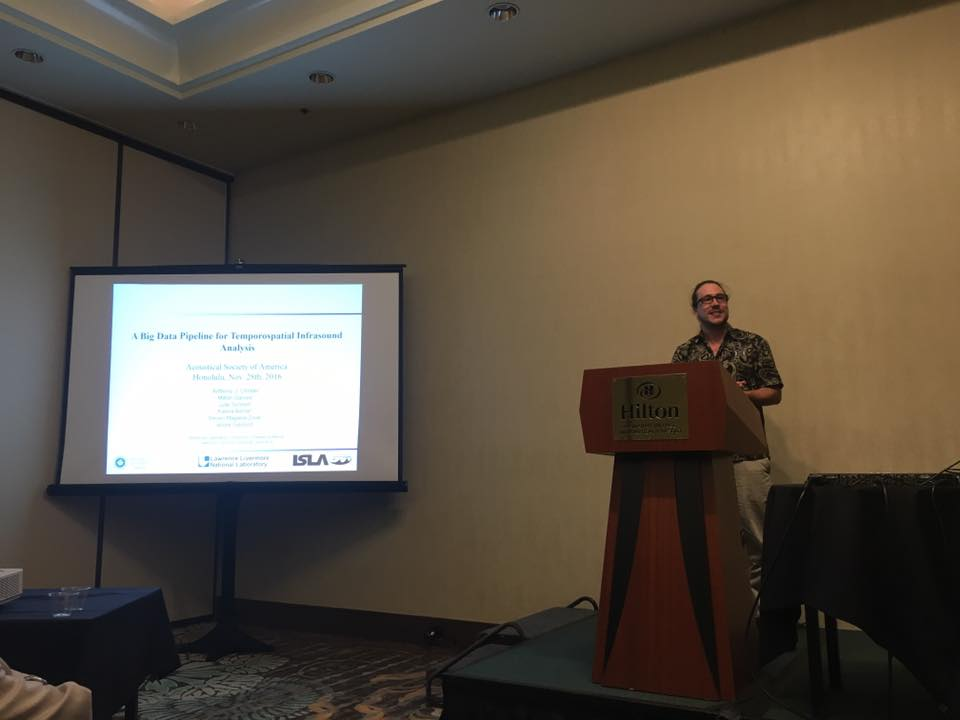
\includegraphics[width=\linewidth]{img/conference.jpg}
		\end{figure}
		\begin{figure}
			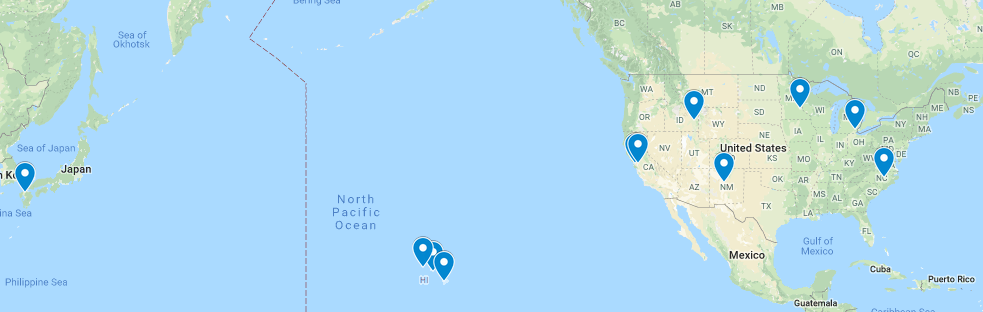
\includegraphics[width=\linewidth]{img/doublebutt.png}
		\end{figure}
	\end{column}
\end{columns}
\end{frame}

\begin{frame}{Ph.D.}
\begin{itemize}
	\item Requires novel contributions to science
	\item Strictly research
	\item A lot of writing and presenting
%	\item General Ph.D. timeline
%	\begin{itemize}
%		\item Acceptance
%		\item Qualifying Exam
%		\item Portfolio
%		\item \textbf{Proposal}
%		\item Dissertation
%		\item Defense
%	\end{itemize}
\end{itemize}
\end{frame}

\section{Computer Science}

\begin{frame}{Is Computer Science Right for You?}
\begin{columns}
	\begin{column}{.50\textwidth}
	\begin{itemize}
		\item Strong communication skills?
		\item Enjoy working in a team?
		\item Want to work in multiple disciplines?
		\item Like solving puzzles?
		\item Mathematically minded?
		\item Enjoy learning?
	\end{itemize}
	\end{column}
\begin{column}{.50\textwidth}
	\begin{figure}
		
\includegraphics[width=\linewidth]{img/noidea.jpg}
	\end{figure}
\end{column}
\end{columns}
\end{frame}

\begin{frame}{Computer Science is \emph{not}...} 
\centering 
\includegraphics[width=.5\linewidth]{img/fortnite.jpg}
\end{frame}

%\begin{frame}{Computer Science is...}
%\begin{itemize}
%\item Computer Science \emph{is}
%\begin{itemize}
%	\item Algorithms
%	\item Data structures
%	\item Software Engineering
%	\item Operating Systems
%	\item Artificial Intelligence
%	\item Mathematical
%	\item ...
%	\item \emph{Social}
%\end{itemize}
%\end{itemize}
%\end{frame}
%
%\begin{frame}
%\begin{figure}
%
\includegraphics[width=\linewidth]{img/all_the_things.jpg}
%\end{figure}
%\end{frame}

\begin{frame}{A Brief Tour of Computer Science}
\begin{itemize}
	\item Computer science is a broad subject consisting of many and varied subfields....
	\item Computer science is
	\begin{itemize}
		\item Part theory
		\item Part application
		\item A lot of art
	\end{itemize}
\end{itemize}
\end{frame}

\begin{frame}{Mobile Applications}
\begin{columns}
	\begin{column}{.40\textwidth}
		\begin{itemize}
			\item iOS, Android development
			\item VR / AR
			\item Mobile gaming
		\end{itemize}
	\end{column}
	\begin{column}{.60\textwidth}
		\begin{figure}
			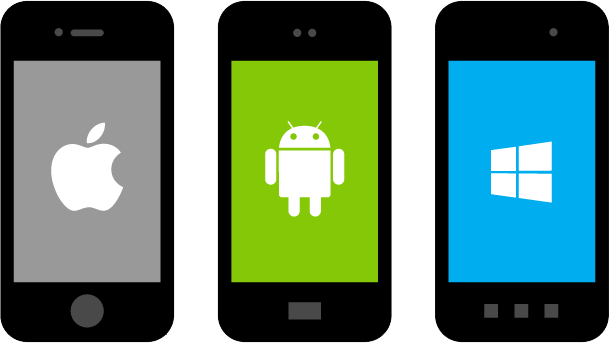
\includegraphics[width=\linewidth]{img/appdev1.png}
		\end{figure}
		\begin{figure}
			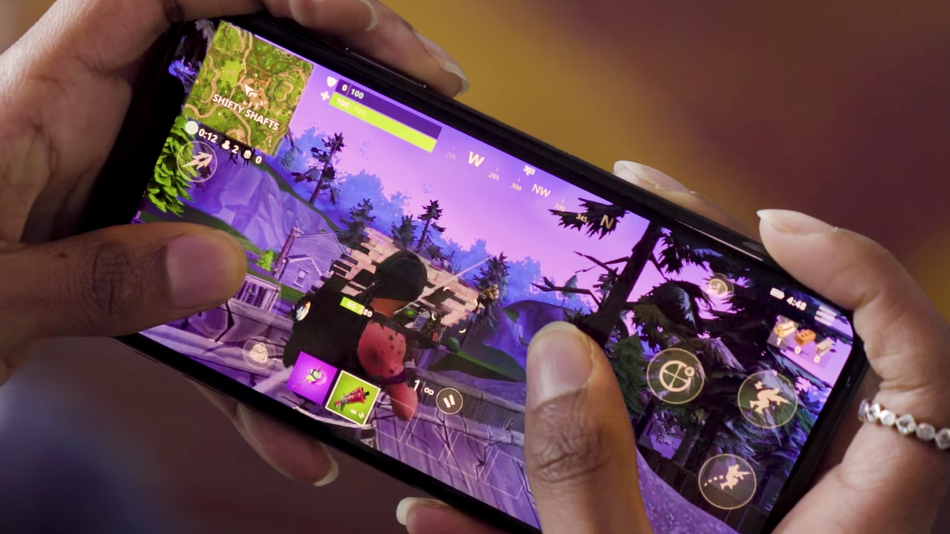
\includegraphics[width=\linewidth]{img/fnapp.png}
		\end{figure}
	\end{column}
\end{columns}
\end{frame}

\begin{frame}{Artificial Intelligence (AI)}
\begin{columns}
	\begin{column}{.40\textwidth}
		\begin{itemize}
			\item Teaching computers how to learn
			\item Automatically recognizing patterns in images, sounds, data sets
			\item Deep learning / neural networks
			\item Autonomous robots
		\end{itemize}
	\end{column}
	\begin{column}{.60\textwidth}
		\begin{figure}
			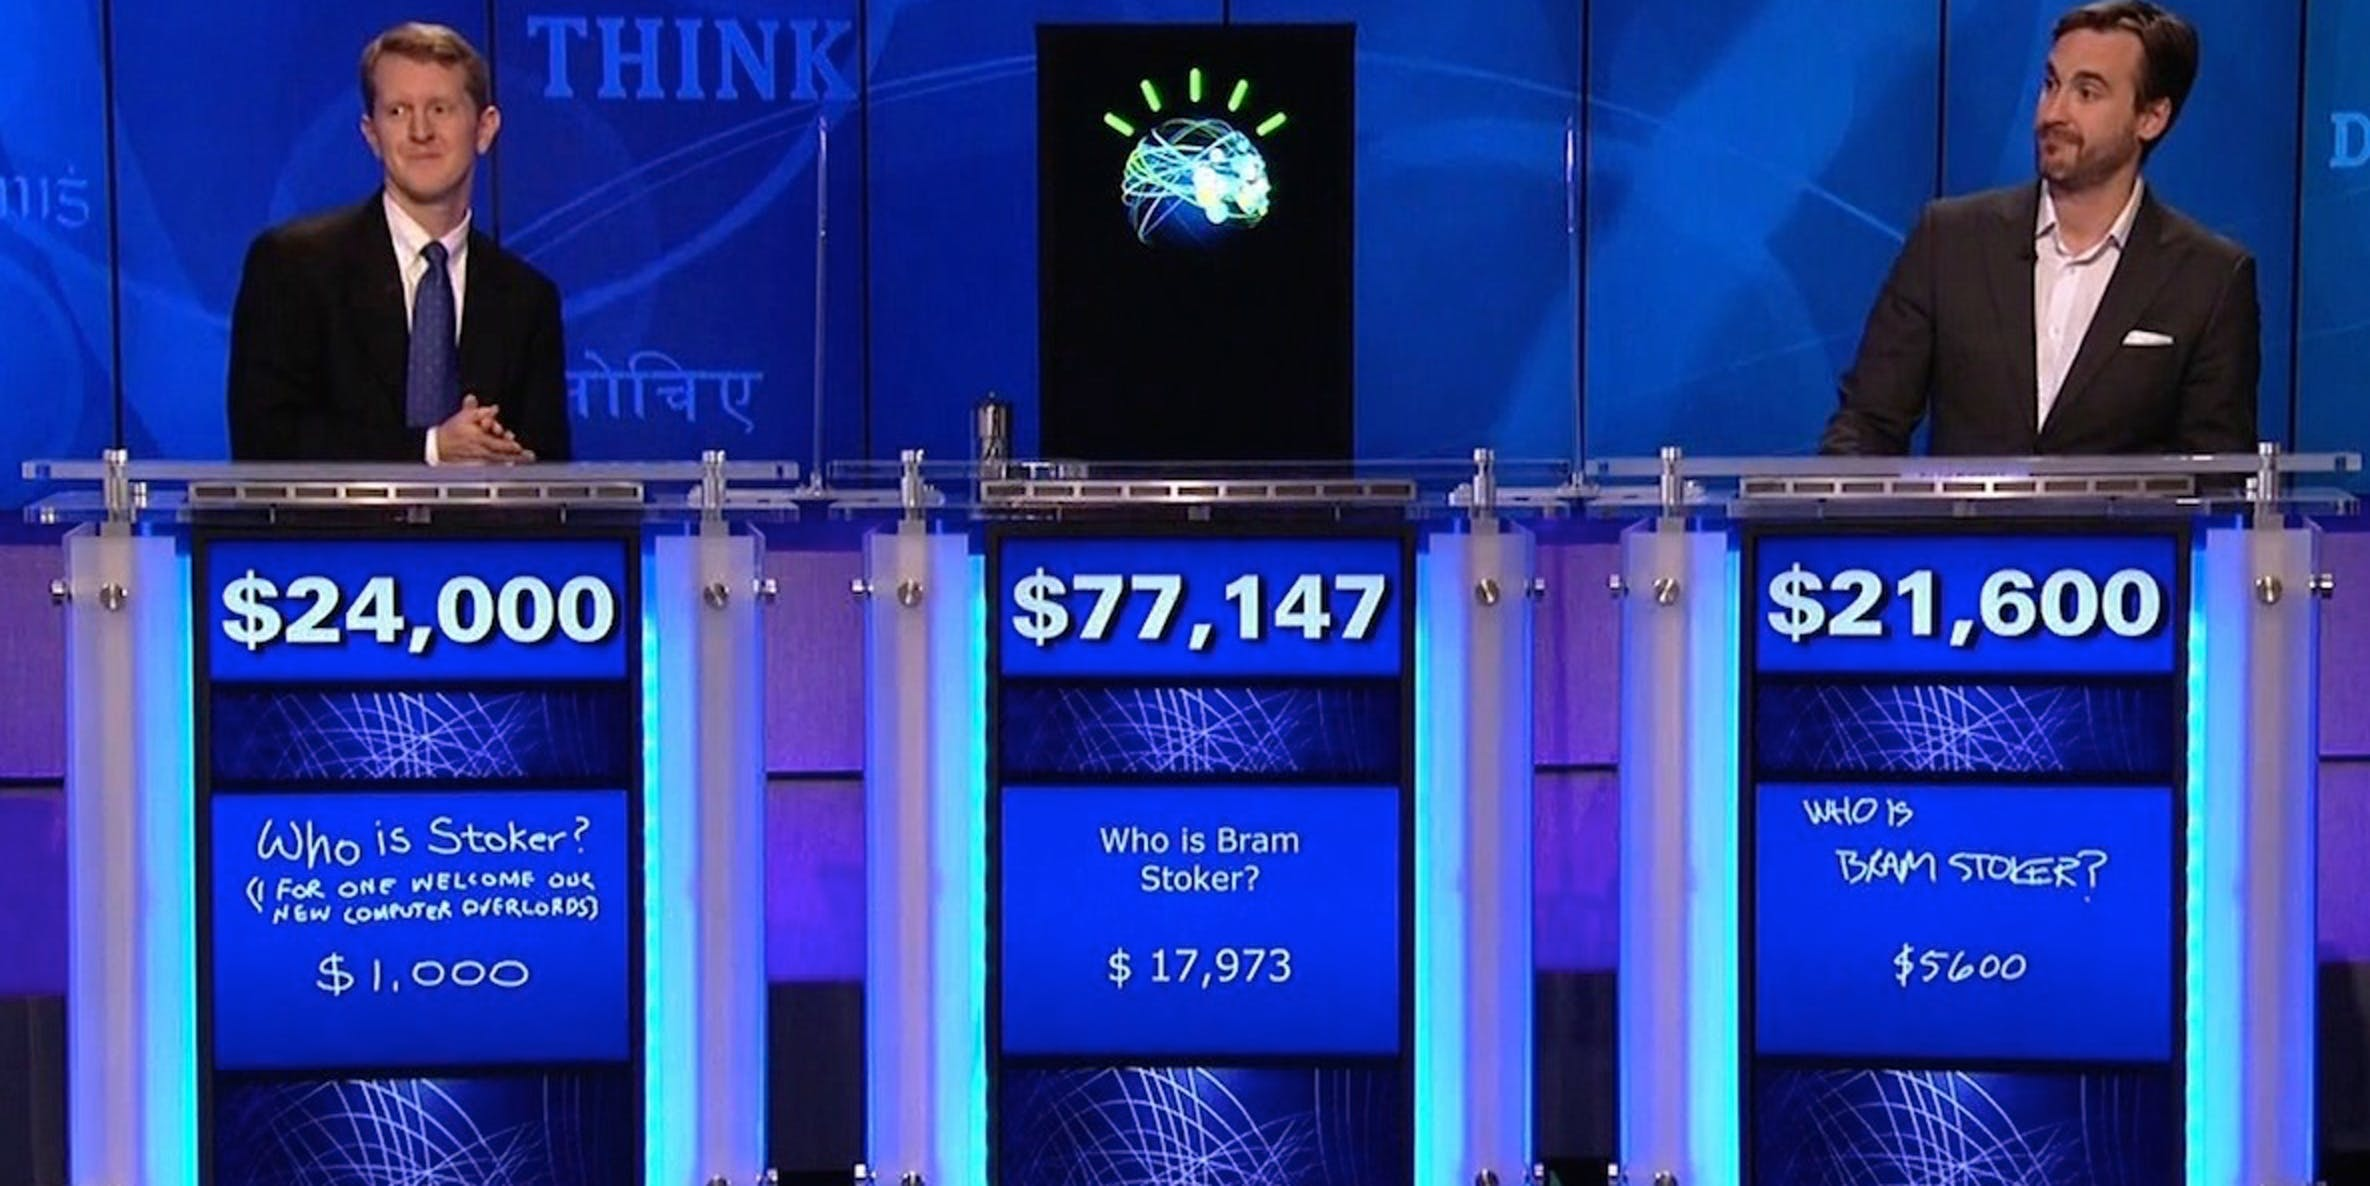
\includegraphics[width=\linewidth]{img/watson.jpg}
		\end{figure}
	\end{column}
\end{columns}
\end{frame}

\begin{frame}{Bioinformatics}
\begin{columns}
	\begin{column}{.45\textwidth}
		\begin{itemize}
			\item Study of biological data
			\item Cyberphysical systems 
		\end{itemize}
	\end{column}
	\begin{column}{.55\textwidth}
		\begin{figure}
			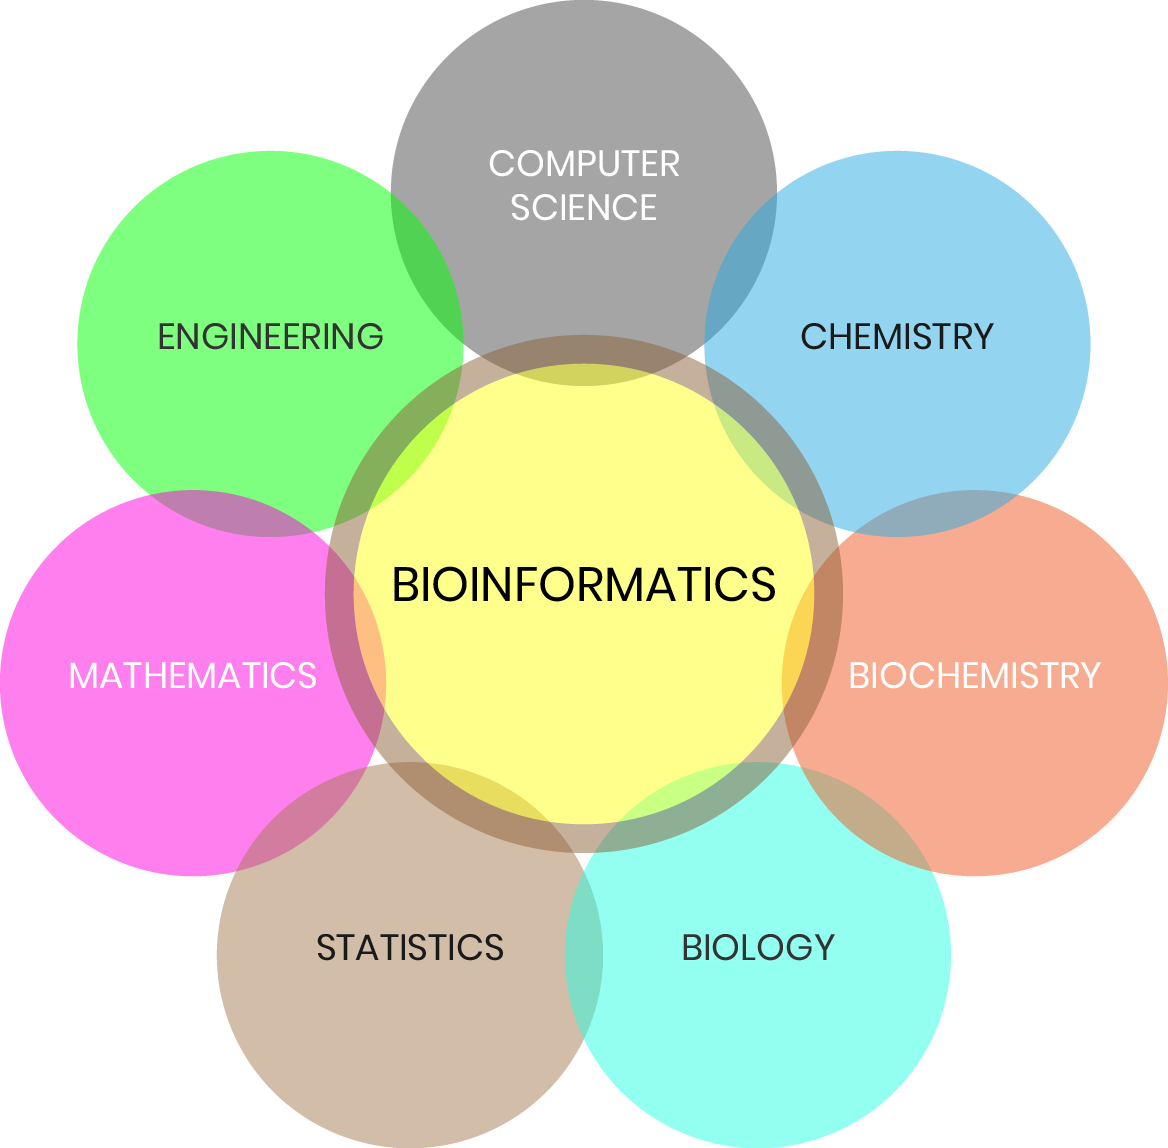
\includegraphics[width=1\linewidth]{img/bio.png}
		\end{figure}
	\end{column}
\end{columns}
\end{frame}

\begin{frame}{Computer Architecture}
\begin{columns}
	\begin{column}{.40\textwidth}
		\begin{itemize}
			\item Hardware design
			\item Processor design
			\item Microcontrollers
			\item Electronics
		\end{itemize}
	\end{column}
	\begin{column}{.60\textwidth}
		\begin{figure}
			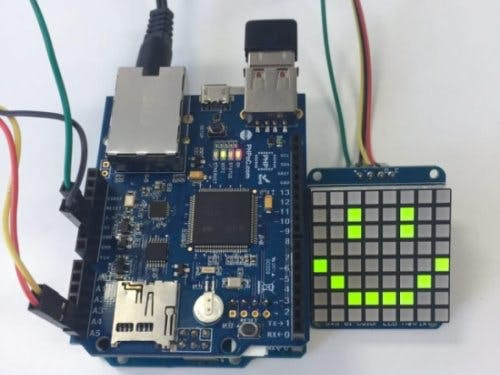
\includegraphics[width=\linewidth]{img/smiley.jpg}
		\end{figure}
	\end{column}
\end{columns}
\end{frame}

\begin{frame}{Computer Graphics and Visualization}
\begin{columns}
	\begin{column}{.40\textwidth}
		\begin{itemize}
			\item Design plots and other visualizations for large data sets
			\item Virtual Reality / Augmented Reality
			\item Video games
		\end{itemize}
	\end{column}
	\begin{column}{.60\textwidth}
		\begin{figure}
			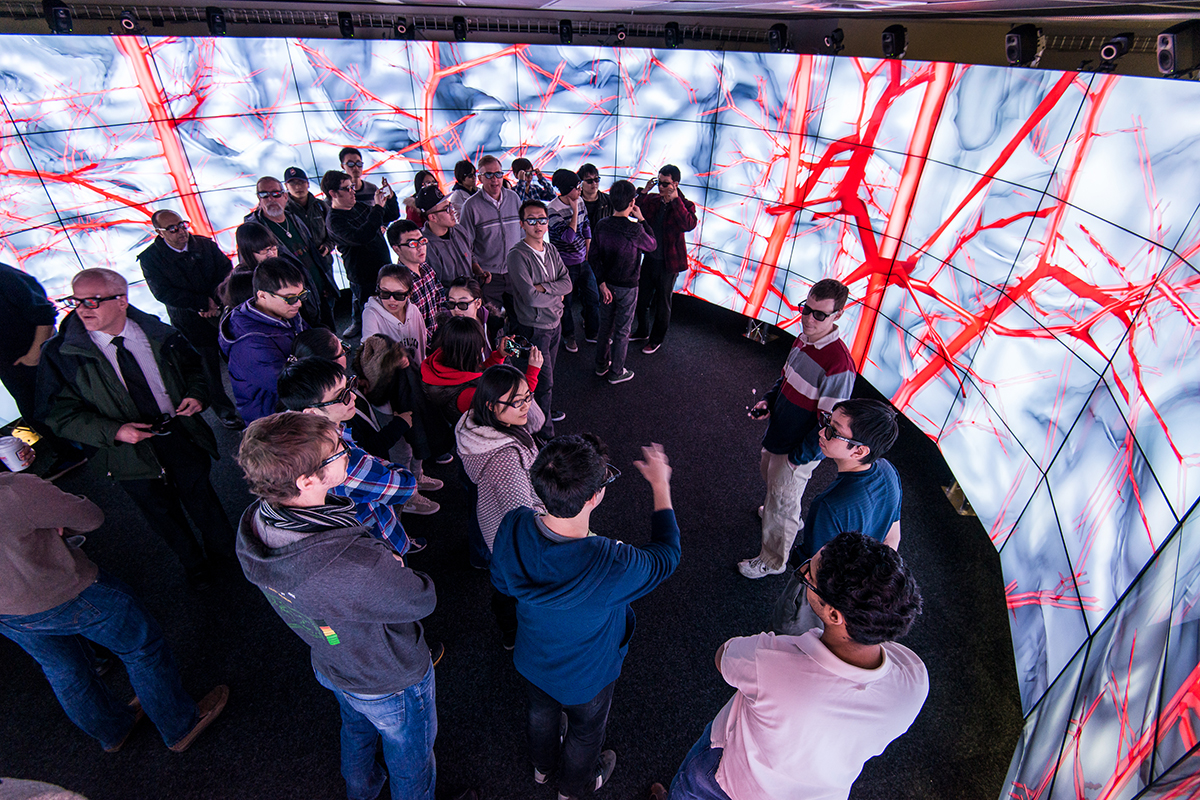
\includegraphics[width=\linewidth]{img/vis.jpg}
		\end{figure}
	\end{column}
\end{columns}
\end{frame}

\begin{frame}{Computer Networks}
\begin{columns}
	\begin{column}{.45\textwidth}
		\begin{itemize}
			\item How computers communicate with each other
			\item Secure communications
			\item The design of the internet
			\item Distributed sensor networks / mobile networks
		\end{itemize}
	\end{column}
	\begin{column}{.55\textwidth}
		\begin{figure}
			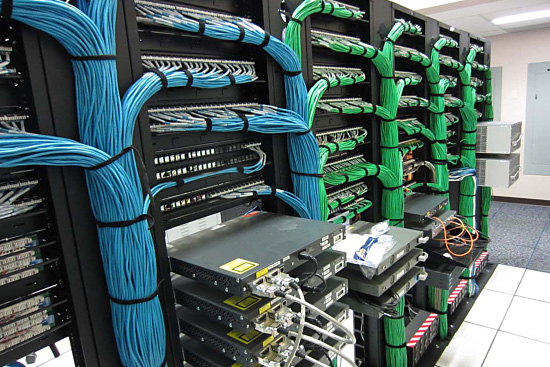
\includegraphics[width=\linewidth]{img/cables.jpg}
		\end{figure}
	\end{column}
\end{columns}
\end{frame}

\begin{frame}{Computer Security}
	\begin{columns}
		\begin{column}{.45\textwidth}
			\begin{itemize}
				\item Both theoretical and practical
				\item Penetration testing
				\item Security protocols
				\item Cryptography (encryption / decryption)
			\end{itemize}
		\end{column}
		\begin{column}{.55\textwidth}
			\begin{figure}
				
\includegraphics[width=\linewidth]{img/hacker.jpg}
			\end{figure}
		\end{column}
	\end{columns}
\end{frame}

\begin{frame}{Databases}
	\begin{columns}
		\begin{column}{.45\textwidth}
			\begin{itemize}
				\item How data is stored and structured
				\item How data is efficiently looked up
				\item More often dealing with Big Data
			\end{itemize}
		\end{column}
		\begin{column}{.55\textwidth}
			\begin{figure}
				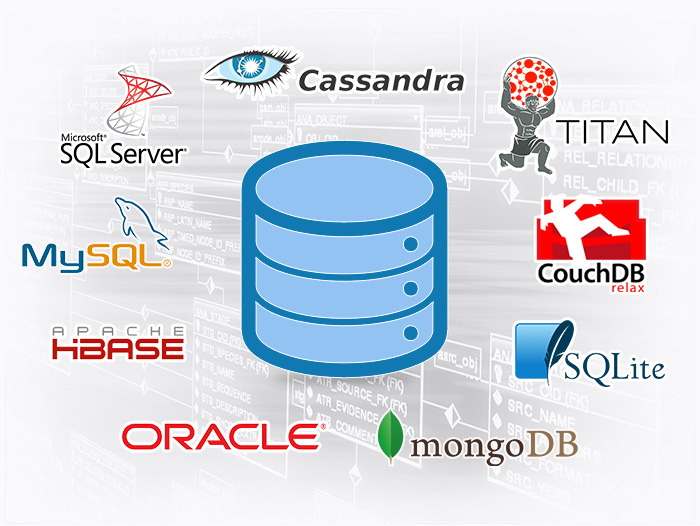
\includegraphics[width=\linewidth]{img/db.jpg}
			\end{figure}
		\end{column}
	\end{columns}
\end{frame}

\begin{frame}{Data Science}
\begin{columns}
	\begin{column}{.45\textwidth}
		\begin{itemize}
			\item Extract knowledge and insights from both structured and unstructured data
			\item Make sense of the large amounts of data being produced
		\end{itemize}
	\end{column}
	\begin{column}{.55\textwidth}
		\begin{figure}
			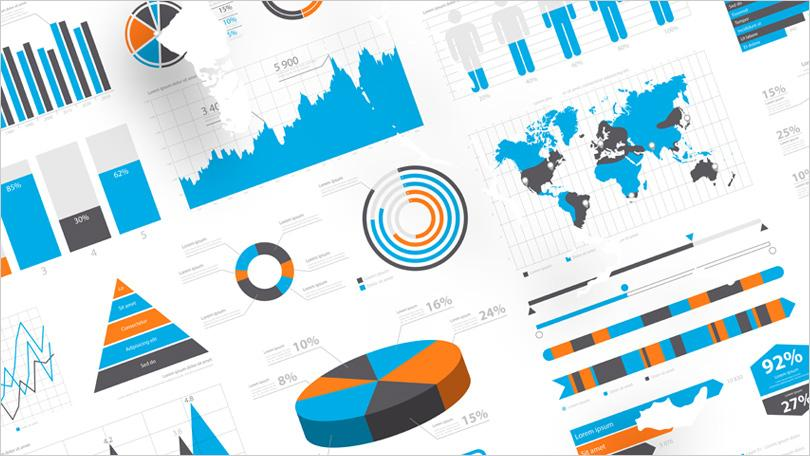
\includegraphics[width=\linewidth]{img/datascience.png}
		\end{figure}
	\end{column}
\end{columns}
\end{frame}

\begin{frame}{Game Design}
\begin{columns}
	\begin{column}{.45\textwidth}
		\begin{itemize}
			\item Multidisciplinary
			\item Software engineering, art design, sound design, networking, testing, graphics design
			\item \emph{A lo}t of math (mainly linear algebra)
		\end{itemize}
	\end{column}
	\begin{column}{.55\textwidth}
		\begin{figure}
			
\includegraphics[width=\linewidth]{img/mc.jpg}
		\end{figure}
	\end{column}
\end{columns}
\end{frame}

\begin{frame}{High Performance Computing (HPC)}
\begin{columns}
	\begin{column}{.45\textwidth}
		\begin{itemize}
			\item Parallel algorithm design
			\item Distributed computations and optimizations
			\item Distributed data storage and access
			\item Simulations 
			\item U.H. Manoa is really good in this
		\end{itemize}
	\end{column}
	\begin{column}{.55\textwidth}
		\begin{figure}
			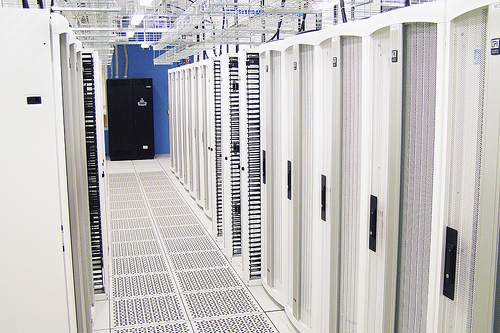
\includegraphics[width=\linewidth]{img/uhsuper.jpg}
		\end{figure}
	\end{column}
\end{columns}
\end{frame}

\begin{frame}{Human Computer Interaction (HCI)}
\begin{columns}
	\begin{column}{.45\textwidth}
		\begin{itemize}
			\item Study of how humans interact with technology
			\item UI/UX  Design
			\item Psychology
			\item Sociology
		\end{itemize}
	\end{column}
	\begin{column}{.55\textwidth}
		\begin{figure}
			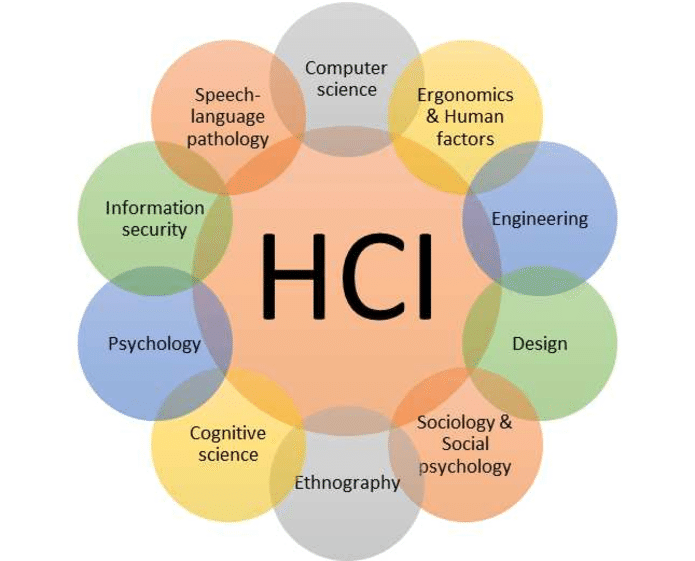
\includegraphics[width=\linewidth]{img/hci.png}
		\end{figure}
	\end{column}
\end{columns}
\end{frame}

\begin{frame}{Robotics}
\begin{columns}
	\begin{column}{.45\textwidth}
		\begin{itemize}
			\item Multidisciplinary
			\begin{itemize}
				\item Computer vision / image processing
				\item A.I. 
				\item Computer architecture
				\item Data science
				\item Very math heavy!
			\end{itemize}
		\end{itemize}
	\end{column}
	\begin{column}{.55\textwidth}
		\begin{figure}
			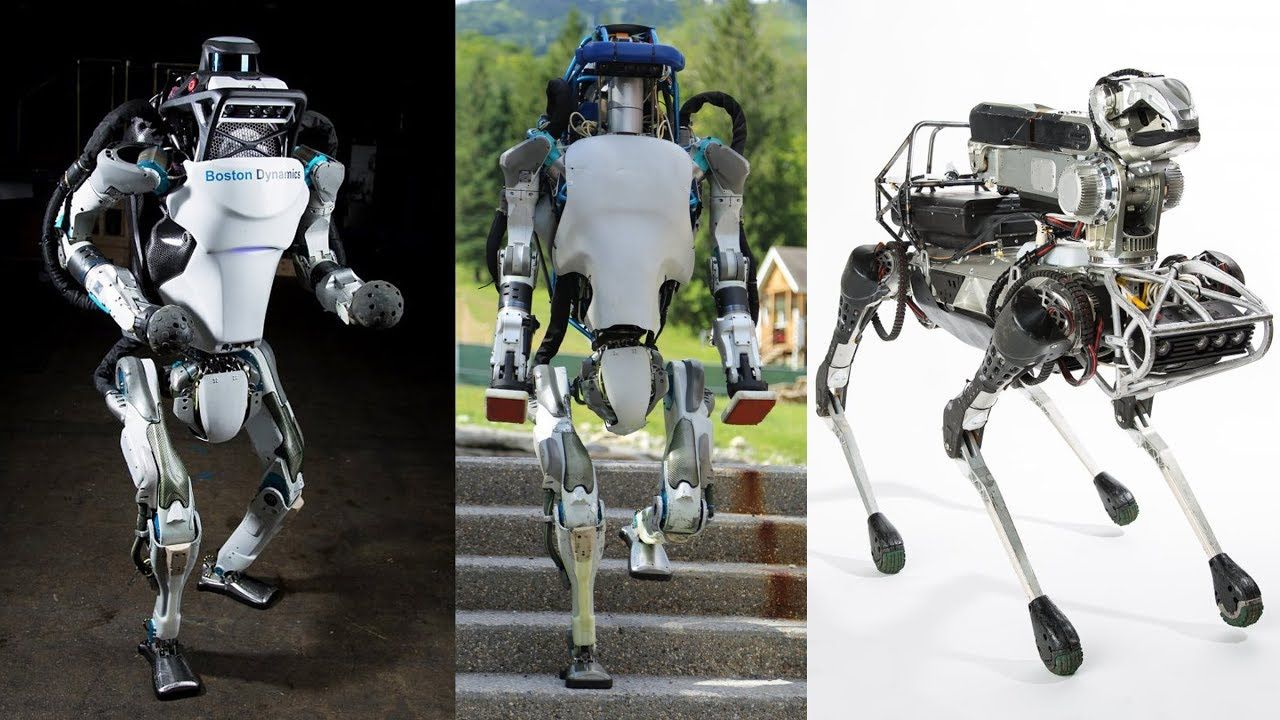
\includegraphics[width=\linewidth]{img/robot.jpg}
		\end{figure}
	\end{column}
\end{columns}
\end{frame}
%
\begin{frame}{Software Engineering}
\begin{columns}
	\begin{column}{.45\textwidth}
		\begin{itemize}
			\item Design and structure of large software systems
			\item Building reliable systems
			\item Methods and best practices for designing software
		\end{itemize}
	\end{column}
	\begin{column}{.55\textwidth}
		\begin{figure}
			
\includegraphics[width=\linewidth]{img/softeng.png}
		\end{figure}
	\end{column}
\end{columns}
\end{frame}

\begin{frame}{Web Design}
\begin{columns}
	\begin{column}{.40\textwidth}
		\begin{itemize}
			\item Website design
			\item Web servers
			\item Web applications
			\item Artistic design
		\end{itemize}
	\end{column}
	\begin{column}{.60\textwidth}
		\begin{figure}
			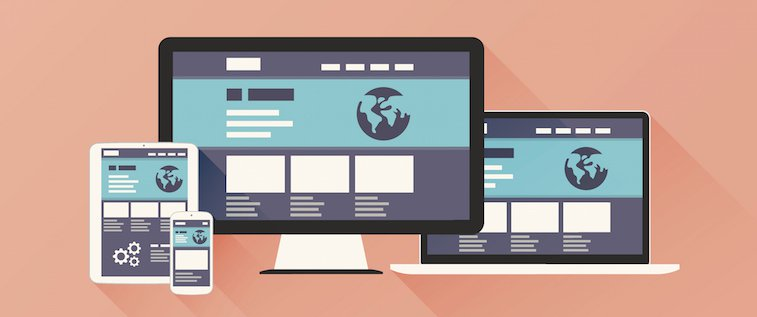
\includegraphics[width=\linewidth]{img/web.jpg}
		\end{figure}
	\end{column}
\end{columns}
\end{frame}

\begin{frame}{And so much more...}
\begin{itemize}
	\item Simulation and modeling
	\item Programming language design
	\item Operating systems
	\item Image processing
	\item Formal methods
	\item Distributed systems
	\item Compiler design
	\item Data structures and algorithms
	\item Theory of computation
\end{itemize}
\end{frame}

\begin{frame}{Picking a career}
\begin{itemize}
	\item Computer science is very multidisciplinary
	\item If you don't know what subfield you're interested in
	\begin{itemize}
		\item Pick a school with a large computer science department
	\end{itemize}
	\item If you do know what subfield you're interested in
	\begin{itemize}
		\item Pick a school that is known for your subfield of choice
	\end{itemize}
	\item If you're interested in staying in Hawaii
	\begin{itemize}
		\item Department of Defense
		\item NSA
		\item Other federal agencies
	\end{itemize}
	\item Military opportunities
\end{itemize}
\end{frame}

\begin{frame}{Thank You!}
\begin{columns}
	\begin{column}{.35\textwidth}
		Anthony Christe \\
		achriste@hawaii.edu
	\end{column}
%	\begin{column}{.65\textwidth}
%		\begin{figure}
%			
\includegraphics[width=\linewidth]{img/meme.png}
%		\end{figure}
%	\end{column}
\end{columns}
\end{frame}

\end{document}
